\section{Evaluation}
\label{eval}

%Evaluation section...
%
%Length: 3-4 pages (graphs take a lot of space!)
%
%Tell reader what to expect.
%
%Eval is "proof" that your design is good.
%MATCH eval goals with design goals.
%
%Eval section is easier to write, but longest one to produce
%results for.  Whereas design section has complex structure, eval
%is more 'flat'.
%
%Structure:
%
%1.  list eval goals, should match design goals
%
%2.  briefly list how you plan to prove those goals.
%
%3.  describe your testbed: h/w + s/w platform to run tests on.
%Give enough detail so it can be reproduced by ANYONE.
%
%4.  describe your benchmarks in detail:
%
%(4a) Micro benchmarks: test specific feature (e.g., read or
%write performance).  Usually u-bench are designed to highlight
%worst/best case behavior of your system.  Be to list both best
%and worst.
%
%(4b) Macro benchmarks (general purpose benchmarks): test whole
%system (e.g., run a Web server exerciser, or TPC for database).
%
%Some tests should compare YOUR system to past systems, or a
%"before and after" comparison.
%
%For every possible variable in your system, design a set of
%independent tests (re: compression study's dimensions).  Justify
%need to vary each variable (the more variables, the more
%experiments you have to run).
%
%5.  Describe your benchmarking methodology
%
%Statistical stability: how many times you run each test? do you
%compute standard deviations, half-width intervals (for student-t
%distribution), RMS, or other metric of stability?  Say how many
%times you ran each test, and what were the stability metrics.
%
%Ex."we ran every test at least 10 times, and computed the
%standard deviation as a percentage of the mean.  In all cases,
%the percentage was less than 5\%, unless otherwise noted."
%
%6.  List every benchmark result, for each test
%
%(a) a graph or table or other figure, plus caption.
%(b) followed by an explanation of the figure: say what one sees
%    in the figure, then explain WHY it is so.
%
%7.  Optional: if eval section longer than usual, end it with a
%one-paragraph summary of eval results.
%%%%%%%%%%%%%%%%%%%%%%%%%%%%%%%%%%%%%%%%%%%%%%%%%%%%%%%%%%%%%%%%%%%%%%%%%%%%%%%
% Table(s) for results of current experiments
%%%%%%%%%%%%%%%%%%%%%%%%%%%%%%%%%%%%%%%%%%%%%%%%%%%%%%%%%%%%%%%%%%%%%%%%%%%%%%

\begin{table*}[th]
\small
\centering
%\begin{tabularx}{\linewidth}{|c|c|c|c|c|c|c|X|}

\begin{tabular}{ c|c|c|c|c|c|c|c|c| }
  \cline{2-9}
  & 
  \multicolumn{2}{c}{\textbf{$u_{1}$}} &
  \multicolumn{2}{|c}{\textbf{$u_{2}$}} &
  \multicolumn{2}{|c}{\textbf{$u_{3}$}} &
  \multicolumn{2}{|c|}{\textbf{root}}  \\
  \cline{2-9}
  \multicolumn{1}{c|}{} &
  with & without & with & without & with & without & with & without\\
  \multicolumn{1}{c|}{} &
  change & changes & changes & changes & changes & changes & changes &
  changes\\
  \hline
  \multicolumn{1}{|c|}{\textbf{create file}}
  & Y & Y & N & Y & N & Y & N & Y \\
  \hline
  \multicolumn{1}{|c|}{\textbf{create dir}}
  & Y & Y & N & Y & N & Y & N & Y \\
  \hline
  \multicolumn{1}{|c|}{\textbf{remove file}}
  & Y & Y & N & Y & N & Y & N & Y \\
  \hline
  \multicolumn{1}{|c|}{\textbf{remove dir}}
  & Y & Y & N & Y & N & Y & N & Y \\
  \hline
  \multicolumn{1}{|c|}{\textbf{create symlink}}
  & Y & Y & N & Y & N & Y & N & Y \\
  \hline
  \multicolumn{1}{|c|}{\textbf{read symlink}}
  & Y & Y & N & Y & N & Y & N & Y \\
  \hline
  \multicolumn{1}{|c|}{\textbf{write symlink}}
  & Y & Y & N & Y & N & Y & N & Y \\
  \hline
  \multicolumn{1}{|c|}{\textbf{create hardlink}}
  & Y & Y & N & Y & N & Y & N & Y \\
  \hline
  \multicolumn{1}{|c|}{\textbf{write hardlink}}
  & Y & Y & N & Y & N & Y & N & Y \\
  \hline
  \multicolumn{1}{|c|}{\textbf{stat}}
  & Y & Y & N & Y & N & Y & N & Y \\
  \hline
  \multicolumn{1}{|c|}{\textbf{change dir}}
  & Y & Y & N & Y & N & Y & N & Y \\
  \hline
  \multicolumn{1}{|c|}{\textbf{read file}}
  & Y & Y & N & Y & N & Y & N & Y \\
  \hline
  \multicolumn{1}{|c|}{\textbf{write file}}
  & Y & Y & N & Y & N & Y & N & Y \\
  \hline
  \multicolumn{1}{|c|}{\textbf{create tar}}
  & Y & Y & N & Y & N & Y & N & Y \\
  \hline
  \multicolumn{1}{|c|}{\textbf{untar}}
  & Y & Y & N & Y & N & Y & N & Y \\
  \hline
  \multicolumn{1}{|c|}{\textbf{make}}
  & Y & Y & N & Y & N & Y & N & Y \\
  \hline
  \multicolumn{1}{|c|}{\textbf{rename}}
  & Y & Y & N & Y & N & Y & N & Y \\
  \hline
\end{tabular}

%\end{tabularx}
\caption{\capfont Results of different file system operations for
different users, with and without the changes.}
\label{tab:results}
\end{table*}

%%%%%%%%%%%%%%%%%%%%%%%%%%%%%%%%%%%%%%%%%%%%%%%%%%%%%%%%%%%%%%%%%%%%%%%%%%%%%%
%% For Emacs:
% Local variables:
% fill-column: 70
% End:
%%%%%%%%%%%%%%%%%%%%%%%%%%%%%%%%%%%%%%%%%%%%%%%%%%%%%%%%%%%%%%%%%%%%%%%%%%%%%%
%% For Vim:
% vim:textwidth=70
%%%%%%%%%%%%%%%%%%%%%%%%%%%%%%%%%%%%%%%%%%%%%%%%%%%%%%%%%%%%%%%%%%%%%%%%%%%%%%
% LocalWords:  PEAFS PEAIO Lustre SBU HMC config

%%%%%%%%%%%%%%%%%%%%%%%%%%%%%%%%%%%%%%%%%%%%%%%%%%%%%%%%%%%%%%%%%%%%%%%%%%%%%%%
% Table(s) for results of current experiments
%%%%%%%%%%%%%%%%%%%%%%%%%%%%%%%%%%%%%%%%%%%%%%%%%%%%%%%%%%%%%%%%%%%%%%%%%%%%%%

\begin{table*}[th]
\small
\centering
%\begin{tabularx}{\linewidth}{|c|c|c|c|c|c|c|X|}

\begin{tabular}{ c|c|c|c|c|c|c| }
  \cline{2-7}
  & 
  \multicolumn{2}{c}{\textbf{root}} &
  \multicolumn{2}{|c}{\textbf{user1}} &
  \multicolumn{2}{|c|}{\textbf{root\_notallowed}}\\ 
  \cline{2-7}
  \multicolumn{1}{c|}{} &
  with & without & with & without & with & without\\
  \multicolumn{1}{c|}{} &
  changes & changes & changes & changes & changes & changes\\
  \hline
  \multicolumn{1}{|c|}{\textbf{xfstests}}
  & 56(68) & 56(68) & 32(68) & 32(68) & 0(68) & - \\
  \hline
  \multicolumn{1}{|c|}{\textbf{eCryptfs-tests}}
  & 25(25) & 25(25) & 22(25) & 22(25) & 0(25) & - \\
  \hline
\end{tabular}

%\end{tabularx}
\caption{\capfont Number of passed tests and total tests for
\emph{XFSTEST} and \emph{eCryptfs-tests} for different users, with and
without the changes.}
\label{tab:results-xfs}
\end{table*}

%%%%%%%%%%%%%%%%%%%%%%%%%%%%%%%%%%%%%%%%%%%%%%%%%%%%%%%%%%%%%%%%%%%%%%%%%%%%%%
%% For Emacs:
% Local variables:
% fill-column: 70
% End:
%%%%%%%%%%%%%%%%%%%%%%%%%%%%%%%%%%%%%%%%%%%%%%%%%%%%%%%%%%%%%%%%%%%%%%%%%%%%%%
%% For Vim:
% vim:textwidth=70
%%%%%%%%%%%%%%%%%%%%%%%%%%%%%%%%%%%%%%%%%%%%%%%%%%%%%%%%%%%%%%%%%%%%%%%%%%%%%%
% LocalWords:  PEAFS PEAIO Lustre SBU HMC config

%
%\paragraph{Evaluation Goals}
%We aimed to provide a correct working solution for eCryptfs with minimal
%performance overheads.
%
%\begin{itemize}
%\item
%\textbf{Correctness}\\
%Only the users that are allowed to access, should be able to access
%the file contents.  Other users should get a permission denied error
%irrespective of their privilege level.
%
%The user who is assigned the administrative role should be able to add
%or revoke permissions to other users in the system.
%
%Users without administrative privilege should not be able to change
%file access policy or gain illegal access.
%\item
%\textbf{Performance}\\ Performance of underlying file system should
%not suffer a penalty due to this extra security enforcement in
%eCryptfs.
%
%We keep the policy management separate from data path, so there is no
%overhead from management tasks on system performance.
%\item
%\textbf{Regression testing}\\ This change should not break any
%existing functionality in eCryptfs as well as the underlying file
%system.
%
%We have tested our changes with basic file operations like create
%file, directory, symlink, delete, rename, untar, kernel compilation.
%We also have run more comprehensive tests such as
%\emph{XFSTESTS}~\cite{xfstests} and eCryptfs-utils test scripts.
%\end{itemize}
%
%\paragraph{Evaluation Plan}
%We have run a set of testing tools along with our manually written
%tests.  The tools are \emph{XFSTESTS} and test scripts provided in
%eCriptfs-utils.  We have run these tools on both modified and
%unmodified eCryptfs kernel for different users with different
%privilege level.  We have tried to run the maximum number of tests
%from these tools, in case of a test failure we rerun it in isolation and
%identify the root cause of failure.  Test cases from these tools are
%sufficient, as they test for the functionality and regression of the file
%system.
%
%\paragraph{Experimental Setup}
%We have used a virtual machine with two Intel\textregistered
%Xeon\texttrademark dual-core 2.40GHz CPUs, and 8GB RAM.  The machine
%ran \mbox{Ubuntu} 14.04.1 with a vanilla 3.19.5 Linux Kernel.  We
%chose \mbox{Ubuntu} because it is freely available and the package
%eCryptfs-utils is installed by default.  For our experiments, we have
%4 users $u_1$, $u_2$, $u_3$ and a root user.  Only user $u_1$ is
%authorized to access encrypted files.  User $u_2$ is placed in sudoer
%list, $u_3$ is a normal user.  All users have intention to access the
%encrypted data, so we have 3 type of attackers and one authorized
%user.
%
%
%\begin{figure}[t]
%    \centering
%    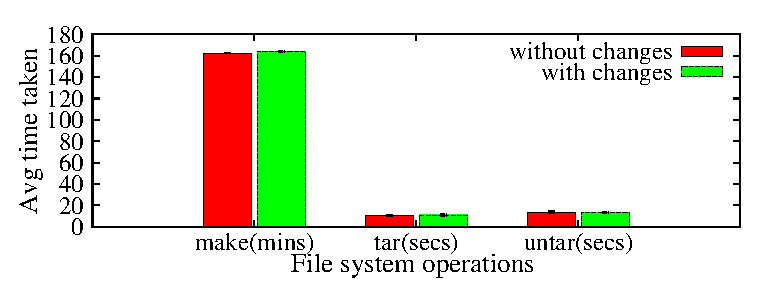
\includegraphics[width=0.5\textwidth]{figures/perf-results.eps}
%    \caption{eCryptfs performance comparison with and without our
%    changes for make, tar, untar operations.}
%    \label{fig:perf-results}
%\end{figure}
%
%
%\paragraph{Results}
%We ran basic file system operation for all four users mentioned above
%on the setup described.  We made changes to Linux Kernel 3.19.5.
%Table~\ref{tab:results} describes the results for all the file systems
%operations we ran.  Column 1 describes the file system operation.
%Column 2,3,4 shows results for users $u_1$, $u_2$, $u_3$ and root user
%respectively with and without our changes in Linux kernel.  \textbf{Y}
%indicates that the  operation ran successfully.  \textbf{N} indicates
%that the user was denied to run the corresponding commands inside the
%eCryptfs mount point.  We also ran some performance tests, such as
%make a Linux Kernel, tar/untar the source tree of Linux Kernel.
%Figure~\ref{fig:perf-results} shows that there is no significant
%performance overhead due to our changes.  The overhead for make workload
%is \emph{1.17\%} and for tar/untar is \emph{1.66\%}.
%
%We ran \emph{XFSTESTS} test-suite on Linux-3.19.5 vanilla kernel for
%\emph{eCryptfs} file system.  We used \emph{FSL} git repository of
%\emph{XFSTESTS} for our tests.  We modified the test-suite to support
%\emph{eCryptfs} file system.  These tests can be categorized in two
%categories, 1, without changes and 2, with changes in eCryptfs kernel
%code.  For category 1 we ran the test-suite for root user and a
%non-root user.  For category 2 we ran the test-suite for an allowed
%non-root user, and root user.  Then we added the root user to allowed
%users list and ran the test-suite again.  We compared the test results
%for both categories for each corresponding user.  We find there is no
%difference in the results.  We see that for category 2, when root user
%was not allowed to access eCryptfs file system, all tests failed.
%
%We also found new interesting bugs with eCryptfs file system.
%\begin{itemize}
%\item 
%\textbf{noatime mount option:} If the eCryptfs file system is mounted
%with noatime mount option, the access times for any file should never
%change.  But we see that there is no difference between if file system
%is mounted with noatime option or not.  The access time for files
%changes in both the cases.
%
%\item
%\textbf{Direct IO:} eCryptfs does not support direct IO.  So all the
%tests for direct IO failed.
%\item
%\textbf{File access timestamp Epoch:} Create a file in eCryptfs
%directory with creation time before epoch.  Check the time of last
%access as seconds since Epoch, it should be a negative value.  Now
%flush the cache by remounting the file system.  Now if we check again
%for the time of last access as seconds since Epoch, it should still be
%negative, but that is not the case here.
%\end{itemize}
%
%All the \emph{XFSTESTS} that failed can be assigned to the issues
%mentioned above.
%
%We also ran the default eCryptfs-test script found in eCryptfs utils.
%These tests include various file systems tests, such as file read,
%write, concurrent access, inode races, symlinks, file truncate.  These
%tests also include tests for already identified bugs in eCryptfs.
%These tests ensures that we did not break anything that was working
%before our changes.  For both the categories, we did not find any
%difference in the results for all the tests.  As expected for any
%non-allowed user all the tests in the script failed.
%
%Table~\ref{tab:results-xfs} shows the number of tests that passed from
%total number of tests for both the test-suites for various users.  We
%examined the failed tests and identified why some of \emph{XFSTESTS}
%failed.  The numbers show that there was nothing broken due to our
%changes.  Since many tests requires root permissions as these are
%kernel level tests, the amount of tests that failed for non-root user
%were considerably higher than that of root user.
%
%IOCTL interface is restricted to admin user.  For our experiments we
%hard coded a UID \mbox{1234} as admin user in eCryptfs kernel.  We
%created a user with UID \mbox{1234} using adduser(1) utility.  At
%mount time only admin user is added to the list of allowed users.
%Root can mount the file system but cannot access the files within the
%mount point, as it is not part of allowed list.  At this point only
%admin user can perform file operation and user management activity.
%Once the admin added a user to the set of allowed users, that user can
%perform file operation.  Still user management operations like
%list\_users/allow\_user/revoke\_user is restricted to admin user.
%
%We tested IOCTL interface via multiple users like admin, user1, user2,
%root.  We observed that only admin user was able to successfully run
%the IOCTL commands, other users including root got permission denied
%error.  Since admin role is non-revocable, even the admin user cannot
%revoke itself.  Admin user cannot add any users to the allowed list
%once the list was full, too many users error is returned.  We verified
%that the file operation path was being properly affected by the
%changes done via IOCTL interface.
%
%%%%%%%%%%%%%%%%%%%%%%%%%%%%%%%%%%%%%%%%%%%%%%%%%%%%%%%%%%%%%%%%%%%%%%%%%%%%%%
%% For Emacs:
% Local variables:
% fill-column: 70
% End:
%%%%%%%%%%%%%%%%%%%%%%%%%%%%%%%%%%%%%%%%%%%%%%%%%%%%%%%%%%%%%%%%%%%%%%%%%%%%%%
%% For Vim:
% vim:textwidth=70
%%%%%%%%%%%%%%%%%%%%%%%%%%%%%%%%%%%%%%%%%%%%%%%%%%%%%%%%%%%%%%%%%%%%%%%%%%%%%%
% LocalWords:
